% ****** Start of file apssamp.tex ******
%
%   This file is part of the APS files in the REVTeX 4.2 distribution.
%   Version 4.2a of REVTeX, December 2014
%
%   Copyright (c) 2014 The American Physical Society.
%
%   See the REVTeX 4 README file for restrictions and more information.
%
% TeX'ing this file requires that you have AMS-LaTeX 2.0 installed
% as well as the rest of the prerequisites for REVTeX 4.2
%
% See the REVTeX 4 README file
% It also requires running BibTeX. The commands are as follows:
%
%  1)  latex apssamp.tex
%  2)  bibtex apssamp
%  3)  latex apssamp.tex
%  4)  latex apssamp.tex
%
\documentclass[%
 reprint,prl, %% for final paper
%superscriptaddress,
%groupedaddress,
%unsortedaddress,
%runinaddress,
%frontmatterverbose, 
%preprint, %% for single-column, double-spacing
%preprintnumbers,
%nofootinbib,
%nobibnotes,
%bibnotes,
 amsmath,amssymb,
 aps,
%pra,
%prb,
%rmp,
%prstab,
%prstper,
%floatfix,
]{revtex4-2}
\usepackage[utf8]{inputenc}
\usepackage{graphicx}% Include figure files
\usepackage{dcolumn}% Align table columns on decimal point
\usepackage{bm}% bold math
\usepackage{hyperref}% add hypertext capabilities
\usepackage[mathlines]{lineno}% Enable numbering of text and display math
\usepackage{amsmath} %for multiline in equation
%\usepackage{comment}

%\linenumbers %for preprint
\relax % Commence numbering lines
%\usepackage[showframe,%Uncomment any one of the following lines to test 
%%scale=0.7, marginratio={1:1, 2:3}, ignoreall,% default settings
%%text={7in,10in},centering,
%%margin=1.5in,
%%total={6.5in,8.75in}, top=1.2in, left=0.9in, includefoot,
%%height=10in,a5paper,hmargin={3cm,0.8in},
%]{geometry}

%abbreviation
\newcommand{\gagg}{\ensuremath{\left|g_{a\gamma\gamma}\right|}}
\newcommand{\ggamma}{\ensuremath{\left|g_{\gamma}\right|}}
\newcommand{\bgagg}{\ensuremath{g_{a\gamma\gamma}}}
\newcommand{\bggamma}{\ensuremath{g_{\gamma}}}
\newcommand{\ma}{\ensuremath{m_a}}
%\def\muev{\ensuremath{\mu~\mathrm{eV}}
\newcommand{\tsys}{\ensuremath{T_\text{sys}}}
\newcommand{\ta}{\ensuremath{T_\text{a}}}
%\newcommand{\muevcc}{\ensuremath{\,\mu\text{e\hspace{-.08em}V\hspace{-0.16em}/\hspace{-0.08em}}c^2}}
\newcommand{\muevcc}{\ensuremath{\,\mu\text{e\hspace{-.08em}V}}}
\newcommand{\MeV}{\ensuremath{\,\text{Me\hspace{-.08em}V}}}
\newcommand{\GeV}{\ensuremath{\,\text{Ge\hspace{-.08em}V}}}
\newcommand{\GeVinv}{\ensuremath{\,\text{Ge\hspace{-.08em}V}^{-1}}}
%\newcommand{\flo}{\ensuremath{4.707504}}
%\newcommand{\fhi}{\ensuremath{4.798147}}
%\newcommand{\mlo}{\ensuremath{19.47}}
%\newcommand{\mhi}{\ensuremath{19.84}}
\newcommand{\flo}{\ensuremath{4.70750}}
\newcommand{\fhi}{\ensuremath{4.79815}}
\newcommand{\mlo}{\ensuremath{19.4687}}
\newcommand{\mhi}{\ensuremath{19.8436}}
\newcommand{\avelimit}{\ensuremath{7.8\times 10^{-14}}}
\newcommand{\lolimit}{\ensuremath{5.0\times 10^{-14}}}
\newcommand{\hilimit}{\ensuremath{8.4\times 10^{-14}}}
% exact number of the average limit 7.6965 x 10^-14 
%\newcommand{\noise}{\ensuremath{2.3}}
\newcommand{\noise}{\ensuremath{1.9 - 2.2}}


\begin{document}

\preprint{APS/123-QED}

\title{First Results from the Taiwan Axion Search Experiment with Haloscope in the \mlo--\mhi\muevcc\ Mass Range}% Force line breaks with \\
\thanks{A footnote to the article title}%

\author{Ann Author}
 \altaffiliation[Also at ]{Physics Department, XYZ University.}%Lines break automatically or can be forced with \\
\author{Second Author}%
 \email{Second.Author@institution.edu}
\affiliation{%
 Authors' institution and/or address\\
 This line break forced with \textbackslash\textbackslash
}%

\collaboration{TASEH Collaboration}%\noaffiliation


\date{\today}% It is always \today, today,
             %  but any date may be explicitly specified

\begin{abstract}

 This Letter reports on the first results from the 
Taiwan Axion Search Experiment with Haloscope, a search for axions 
using a microwave cavity at frequencies between \flo\ and \fhi~GHz. 
Apart from the external signals, no candidates with 
a significance more than 3.355 were found. The experiment excludes 
models with the axion-two-photon 
coupling $\gagg\gtrsim \avelimit\GeVinv$, a factor of ten above the benchmark 
KSVZ model for the mass range $\mlo < \ma < \mhi \muevcc$, reaching 
a sensitivity three orders of magnitude better than any existing limits. 
 It is also the first time that a haloscope-type experiment places 
constraints on the \gagg\ in this mass region.



%\begin{description}
%\item[Usage]
%Secondary publications and information retrieval purposes.
%\item[Structure]
%You may use the \texttt{description} environment to structure your abstract;
%use the optional argument of the \verb+\item+ command to give the category of each item. 
%\end{description}
\end{abstract}

%\keywords{Suggested keywords}%Use showkeys class option if keyword
                              %display desired
\maketitle

%\tableofcontents %for preprint
%%%%%%%%%%%%%%%%%%%%%%%%%%%%%%%%%%%%%%%%%%%%%%%%%%%%%%%%%%%%%%%%%%%%%%%%%%%%%%%
%%% Introduction} 
The axion is a hypothetical particle predicted as a consequence of a  
solution to the strong CP problem~\cite{strongCPI,strongCPII,strongCPIII}. 
The solution proposed by Peccei and Quinn is to introduce a new global 
Peccei-Quinn U(1)$_\mathrm{PQ}$ symmetry that is spontaneously broken; the 
axion is the pseudo Nambu-Goldstone boson of 
U(1)$_\mathrm{PQ}$~\cite{strongCPI}. 
Axions are abundantly produced during the QCD phase transition in 
the early universe and may constitute the dark matter (DM). 
%In the post-inflationary PQ symmetry breaking scenario, where the PQ symmetry
%is broken after inflation, current calculations suggest a mass range of 
%${\cal O}(1–100)$~\muevcc\ for axions so that the cosmic axion density does 
%not exceed the 
%observed cold DM density~\cite{QCDCalI,QCDCalII,QCDCalIII,QCDCalIV,QCDCalV,QCDCalVI,QCDCalVII,QCDCalVIII,QCDCalIX,QCDCalX,QCDCalXI,QCDCalXII,QCDCalXIII}. 
%Therefore, axions are compelling because they may explain at the same 
%time two puzzles that are on scales different by more than thirty orders of 
%magnitude. 
%
Axions could be detected and studied via their two-photon interaction, the
so-called ``inverse Primakoff effect''. 
The detectors with the best sensitivities to axions with a mass of 
$\ma\approx \muevcc$, as first put forward by 
Sikivie~\cite{SikivieI,SikivieII},  
are haloscopes consisting of a microwave cavity immersed in a strong static 
magnetic field and operated at a cryogenic temperature. 
In the presence of an external magnetic field, the ambient oscillating axion 
field drives the cavity and they resonate when the frequencies of the 
electromagnetic 
modes in the cavity match the microwave frequency $f$, where $f$ is set by 
the total energy of the axion: $hf=E_a=\ma c^2 + \frac{1}{2}\ma v^2$. The 
axion signal power is further delivered 
to the readout probe followed by a low-noise linear amplifier. 
The axion mass is unknown, therefore, 
the cavity resonator must allow the possibility to be tuned through a range
of possible axion masses. 

The Axion Dark Matter eXperiment (ADMX) excluded the KSVZ 
benchmark model within the mass range of 
1.9--4.2\muevcc\ and the DFSZ benchmark model for the mass ranges 
of 2.66--3.31 and 3.9--4.1\muevcc, 
respectively~\cite{ADMXI,ADMXII,ADMXIII,ADMXIV,ADMXV,ADMXVI,ADMXVII}. 
The Haloscope at Yale Sensitive to Axion Cold dark matter 
(HAYSTAC) had performed searches first for the mass range of 
23.15--24\muevcc\ and later at around 17\muevcc; they excluded axions 
with $\ggamma\geq 1.38 \ggamma^\text{KSVZ}$ for $m_a=16.96-17.12$ and 
17.14--17.28\muevcc~\cite{HAYSTACI}. The Center 
for Axion and Precision Physics Research (CAPP) constructed 
and ran simultaneously several experiments targeting at 
different frequencies; they have pushed the limits towards the 
KSVZ value within a narrow mass region of 
10.7126--10.7186\muevcc~\cite{CAPPI}.
The QUest for AXions-$a\gamma$ (QUAX-$a\gamma$) also pushed their limits 
close to the upper bound of the QCD axion-two-photon couplings for 
$m_a\approx43\muevcc$~\cite{QUAX}.   
%
This Letter presents the first results 
of a search for axions for the mass range of \mlo--\mhi\muevcc, 
from the Taiwan Axion Search Experiment with Haloscope (TASEH). 


%%%%%%%%%%%%%%%%%%%%%%%%%%%%%%%%%%%%%%%%%%%%%%%%%%%%%%%%%%%%%%%%%%%
%\subsection{The expected axion signal power and signal line shape}
%\label{sec:introsignal}

The signal power extracted from a microwave cavity on resonance is given 
by:
\begin{equation}
P_s = \left(\bggamma^2\frac{\alpha^2\hbar^3c^3\rho_a}{\pi^2\Lambda^4}\right)\times
\left(\omega_c\frac{1}{\mu_0}B_0^2VCQ_L\frac{\beta}{1+\beta}\right).
\label{eq:ps}
\end{equation}
The first set of parentheses contains physical constants, 
a dimensionless model-dependent parameter \bggamma, and 
the local dark-matter density 
$\rho_a=0.45~\GeV/\mathrm{cm}^3$~\cite{[{}][{. Both $0.45~\GeV/\mathrm{cm}^3$ 
(used by ADMX, HAYSTAC, CAPP, and QUAX-$a\gamma$) and $0.3~\GeV/\mathrm{cm}^3$ 
(more commonly cited by the direct DM search experiments) are consistent 
with the recent measurements.}]Read:2014qva,PDG}. 
The numerical values of \bggamma\ are -0.97 and 0.36 
in the Kim-Shifman-Vainshtein-Zakharov (KSVZ)~\cite{KSVZI,KSVZII} and 
the Dine-Fischler-Srednicki-Zhitnitsky (DFSZ)~\cite{DFSZI,DFSZII} benchmark 
models, respectively. For the QCD axions, the coupling constant \bgagg\ that 
describes the strength of the axion-two-photon interaction in the Lagrangian 
is related to \bggamma\ and the axion mass \ma: 
\begin{equation}
 \bgagg = \left(\frac{\bggamma\alpha}{\pi \Lambda^2}\right)\ma, 
\label{eq:grelation}
\end{equation}
where $\alpha$ is the 
fine-structure constant and  $\Lambda=78~\MeV$ is a scale parameter that can 
be derived from the mass and the decay constant of the pion and the ratio of 
the up to down quark masses. 
%
The second set of parentheses contains parameters related to the experimental 
setup: the angular resonant frequency of the cavity $\omega_c$, 
the vacuum permeability $\mu_0$, the nominal strength of the external magnetic 
field $B_0$, the volume of the cavity $V$, and the loaded quality factor of 
the cavity \(Q_L=Q_0/(1+\beta)\), where $Q_0$ is the unloaded, intrinsic 
quality factor of the cavity and $\beta$ is the coupling coefficient which 
determines the amount 
of coupling of the signal to the receiver. The form factor $C$ is the 
normalized overlap of the electric field 
$\vec{\bm{E}}$, for a particular cavity resonant mode, with the external 
magnetic field $\vec{\bm{B}}$:
\begin{equation}
  C = \frac{\left[\int\left( \vec{\bm{B}}\cdot\vec{\bm{E}}\right) d^3\bm{x}\right]^2}{B_0^2V\int E^2 d^3\bm{x}}.
\label{eq:formfactor} 
\end{equation} 
Here, the magnetic field $\vec{\bm{B}}$ points mostly along the axial 
direction of the cavity. The field strength has a small variation along the 
radial and axial directions and $B_0=8$~Tesla is the nominal magnetic 
field strength. 
For cylindrical cavities, the largest form factor is from the 
TM$_{010}$ mode. The expected signal power derived from the experimental 
parameters of TASEH is $P_s\simeq 1.5\times10^{-24}$~W for a KSVZ axion 
with a mass of 19.5\muevcc. 

In the axion experiments, the figure of merit that determines the design of 
the experimental setup is the signal-to-noise ratio
(SNR), i.e. the ratio of the signal power $P_s$ to the fluctuation in 
the averaged noise power spectrum $\sigma_n$. 
According to Dicke's Radiometer Equation~\cite{Dicke}, the $\sigma_n$ 
is given by: 
\begin{equation}
 \sigma_n  =  k_B\tsys\sqrt{\frac{\Delta f}{t}} 
 \label{eq:sigman}
\end{equation}
where \tsys\ is the system noise temperature, an effective 
temperature associated with the total noise of the system, 
$t$ is the data integration time $t$ 
and $\Delta f$ is the bandwidth over which a single measurement is made. 
The SNR will therefore be: 
\begin{eqnarray}
   \text{SNR} & = & \frac{P_s}{\sigma_n}, \nonumber \\
              & = & \frac{P_s}{k_B\tsys}\sqrt{\frac{t}{\Delta f}},
 \label{eq:SNR}
\end{eqnarray}  
One could see that the SNR is maximized by an experimental setup with 
a strong magnetic field, a large cavity volume, an efficient cavity 
resonant mode, a receiver with low system noise temperature, and a 
long integration time. 

The system noise temperature \tsys\ has two major components:
\(\tsys = T_\text{cn}  + \ta\) that correspond to the effective
temperatures of the following noise sources: (i)
$T_\text{cn}=\left(\frac{1}{e^{\left.hf\middle/k_BT_\mathrm{c}\right.}-1} 
+ \frac{1}{2}\right)\left. hf\middle/k_B\right.$, the blackbody
radiation from the cavity at a physical temperature $T_\mathrm{c}$ and
the quantum noise associated with the zero-point fluctuation of the
vacuum, which are further modulated by a Lorentzian function due to the
higher temperature at the cavity with respect to that in the
dilution refrigerator.
More details may be found in Ref.~\cite{TASEHAnalysis}. (ii) \ta, the
noise added by the receiver (mainly from the first-stage amplifier).
The Lorentzian modulation of $T_\text{cn}$ will be removed from
the averaged noise spectrum and only the average value of $T_\text{cn}$ 
will be used in the final analysis.
%
Using the operation parameters of TASEH and 
the results from the calibration of readout electronics, 
%the values of $T_\text{b}$, $T_\text{qn}$, and \ta\ are estimated to be about 
%0.07~K, 0.12~K, and \noise~K, respectively.  
%Therefore, 
the value of \tsys\ for TASEH is about 2.0--2.3~K. 

%% Experimental Setup 
The detector of TASEH is located at the Department of Physics, National 
Central University, Taiwan and housed within a cryogen-free dilution 
refrigerator (DR) from BlueFors. A superconducting solenoid 
with a 
bore diameter of 76~mm and a length of 240 mm is integrated with the DR. 
%
The data for the analysis presented here were collected by TASEH 
from October 13, 2021 to November 15, 2021, and termed as the CD102 data, 
where CD stands for ``cool down''. 
During the data taking, the cavity sat in the center of the magnet bore 
and was connected via holders to the mixing flange of the DR at a 
temperature of $T_{\rm mx}\simeq27$~mK. 
The temperature of the cavity stayed at $T_\text{c}\simeq155$~mK, higher 
with respect to the 
DR; it is believed that the cavity had an accidental thermal contact with the 
radiation shield in the DR. 
The cavity, made of oxygen-free high-conductivity (OFHC) copper, has an 
effective volume of $V=0.234$~L and is a two-cell cylinder split along 
the axial direction. 
The cylindrical cavity has an inner radius of 2.5~cm and a 
height of 12~cm.  In order to maintain a smooth surface, the cavity underwent 
the processes of annealing, polishing, and chemical cleaning. The resonant 
frequency of the TM$_{010}$ mode can be tuned over the range of 
4.667--4.959~GHz via the rotation of an off-axis OFHC copper tuning rod, from 
the position closer to the cavity wall to the position closer to the cavity 
center. The form factor $C$ for 
the TM$_{010}$ mode varies from 0.64 to 0.69 over the frequency range of 
the CD102 run.  
The intrinsic, unloaded quality factor $Q_0$ at the cryogenic temperature 
($T_\mathrm{c}\simeq 155$~mK) is $\simeq 60000$.


An output probe, made of a 50-$\Omega$ semi-rigid coaxial cable that was 
soldered to an SMA (SubMiniature version A) connector, was inserted into the 
cavity and its depth was set for 
$\beta\simeq2$ since this value maximizes the scan rate, namely the coverage 
of frequency scans for a given amount of time. 
The signal from the output probe was directed to an 
impedance-matched amplification chain. The first-stage amplifier was 
a low noise high-electron-mobility transistor (HEMT) amplifier 
mounted on the 4K flange. 
The signal was further amplified at room temperature via a 
three-stage post-amplifier, and down-converted 
and demodulated to in-phase (I) and quadrature (Q) components and digitized 
by an analog-to-digital converter with a sampling rate of 2~MHz. 

The CD102 data cover the frequency range of \flo--\fhi~GHz. In this Letter, 
all the frequencies in unit of GHz are quoted with five decimal places as the 
absolute accuracy of frequency is $\approx 10$~kHz. It shall be noted that the 
frequency resolution is 1~kHz.  
There were 837 resonant-frequency steps in total, with a frequency difference 
of $\Delta f_\text{s}=95-115$~kHz between the steps. The value of 
$\Delta f_\text{s}$ was kept within 10\% of 105~kHz rather than 
a fixed value, such that the rotation angle of the tuning rod did not need to 
be fine-tuned and the operation time could be minimized; a 10\% variation of 
the $\Delta f_\text{s}$ is found to have no impact on the \gagg\ limits. 
Each resonant-frequency step is denoted as a ``scan'' 
and the data integration time was about 32-42 minutes. The integration 
time was determined based on the target \gagg\ limits and the experimental 
parameters; the variation of the integration 
time aimed to remove the frequency-dependence in the \gagg\ limits caused by   
frequency dependence of the added noise \ta. 

In order to perform a calibration for the amplification chain, 
the HEMT was connected to a heat source (a 50-$\Omega$ resistor) instead of
the cavity;
various values of input currents were sent to the source to change its
temperature monitored by a thermometer. The power from the source
was delivered following the same transmission line as that in the axion
data running. 
The output power is fitted to a first-order polynomial, as a function of
the source temperature, to extract the gain and added noise \ta\ for the
amplification chain. The value of \ta\ is about \noise~K. 
%
A more detailed description of the TASEH detector, the operation of the 
data run, and the calibration of the gain and added noise temperature of the 
whole amplification chain can be found in Ref.~\cite{TASEHInstrumentation}. 




%%% analysis and results

   The analysis of the TASEH CD102 data follows the procedure similar to that 
developed by the HAYSTAC experiment~\cite{HAYSTACII} and the details are 
described in Ref.~\cite{TASEHAnalysis}. The fast Fourier transform (FFT) 
algorithm is performed on the IQ time series data to obtain the 
frequency-domain power spectrum. 
%Apart from the flat baseline as described by
%Eq.~\eqref{eq:pn}, the noise spectrum observed by TASEH has an additional
%component with a Lorentzian shape due to the higher temperature at the
%cavity with respect to that in the DR. 
The Savitzky-Golay (SG) 
filter~\cite{SGFilter} is applied to remove the structure of the background 
in the frequency-domain power spectrum. All the spectra from different 
frequency scans are combined with a weighting algorithm. 
In order to maximize the SNR, a running window of 
five consecutive bins in the combined spectrum is applied and the five bins 
within each window are merged to construct a final spectrum. 
The five frequency bins correspond to the 5-kHz axion signal line width,  
derived from the standard assumption of axion signal line shape as described 
by Eq.~\eqref{eq:simplesignal}. 
This signal line shape is also used when defining the maximum likelihood 
weights for merging: 
\begin{equation}
\mathcal{F}(f, f_a) = \frac{2}{\sqrt{\pi}}\sqrt{f-f_a}\left(\frac{3}{\alpha}\right)^{3/2}
e^{\frac{-3\left(f-f_a\right)}{\alpha}},
\label{eq:simplesignal}
\end{equation}
where $\alpha\equiv  f_a \left<v^2\right>/c^2$. 
Here, the frequency $f$ must be greater or equal to the axion frequency 
$f_a=\left.\ma c^2\middle/h\right.$. 
In this standard assumption of axion signal line shape, 
the DM halo density distribution is assumed 
to be spherically symmetric and close to be isothermal, which results in a 
velocity distribution similar to the Maxwell-Boltzmann distribution. 
Therefore, the variance $\left<v^2\right>$ and the most probable velocity
(speed) $v_p$ are related to each other:
$\left<v^2\right>=3v_p^2/2=$(270~km/s)$^2$, where $v_p=220$~km/s is the local
circular velocity of DM in the galactic rest frame. 



 After the merging, if there were any potential signal with an SNR larger than 
3.355, a rescan would be proceeded to check if it were a real signal 
or a statistical fluctuation. 
The procedure of the CD102 data taking was to perform a rescan after 
covering every 10~MHz; the rescan was done by adjusting the tuning rod of the 
cavity so to match the resonant frequency to the frequency of the candidate. 
In total, 22 candidates with an SNR greater than 3.355 were found. 
Among them, 17 candidates were from the fluctuations because they were gone 
after a few rescans. 
The remaining five candidates, in the frequency ranges of 
4.71017 -- 4.71019~GHz and 4.74730 -- 4.74738~GHz, reached an SNR 
greater or equal to 5 after rescanning. The signals in the second frequency 
range were detected via a portable antenna outside the DR and found 
to come from the instruments in the laboratory, while the signals 
in the first frequency range were weaker but still present after 
turning off the external magnetic field. 
Therefore, these five candidates are considered external signals and 
no limits are placed for the above two frequency ranges.  

%% results
Since no candidates were found after the rescan, the upper limits 
at 95\% confidence level (C.L.) on the \ggamma\ and the 
 \gagg\ are derived by setting the maximum SNR equal to five.  
Figure~\ref{fig:glimit} shows the limits on the axion-two-photon coupling 
\gagg\ and the ratio of the limits on the dimensionless parameter \ggamma\ 
with respect to the KSVZ benchmark value ($\left|g_\text{KSVZ}\right|=0.97$).  
The analysis that merges bins without 
assuming a signal line shape results in $\approx5.5$\% larger values on the 
\gagg\ limits. If a Gaussian signal line shape with an FWHM of 2.5~kHz,  
about half of the axion line width in Eq.~\eqref{eq:simplesignal}, is 
assumed instead, the limits will be $\approx3.8$\% smaller than the central 
results. 
Overall the total relative systematic uncertainty is 
$\approx 4.6\%$, coming from the uncertainties on the loaded quality 
factor $Q_L$, the coupling coefficient $\beta$, the added noise temperature 
\ta, the effect of the misalignment between the true axion frequency and 
the lower boundaries of the frequency bins, and the variation of the 
SG-filter parameters. 
The limits on 
\gagg\ range from \lolimit\GeVinv\ to \hilimit\GeVinv, with an average 
value of \avelimit\GeVinv; the lowest value comes from the frequency bins with 
additional eight times more data from the rescans, while the highest value 
comes from the frequency bins near the boundaries of the spectrum. 
Figure~\ref{fig:gaggall} displays the \gagg\ limits obtained by TASEH 
together with those from the previous searches. 
The results of TASEH exclude the models with the axion-two-photon
coupling $\gagg\gtrsim \avelimit\GeVinv$, a factor of ten above the benchmark
KSVZ model for the mass range $\mlo < \ma < \mhi \muevcc$ (corresponding to 
the frequency range of $\flo < f_a < \fhi$~GHz). 





\begin{figure*} [htbp]
  \centering
  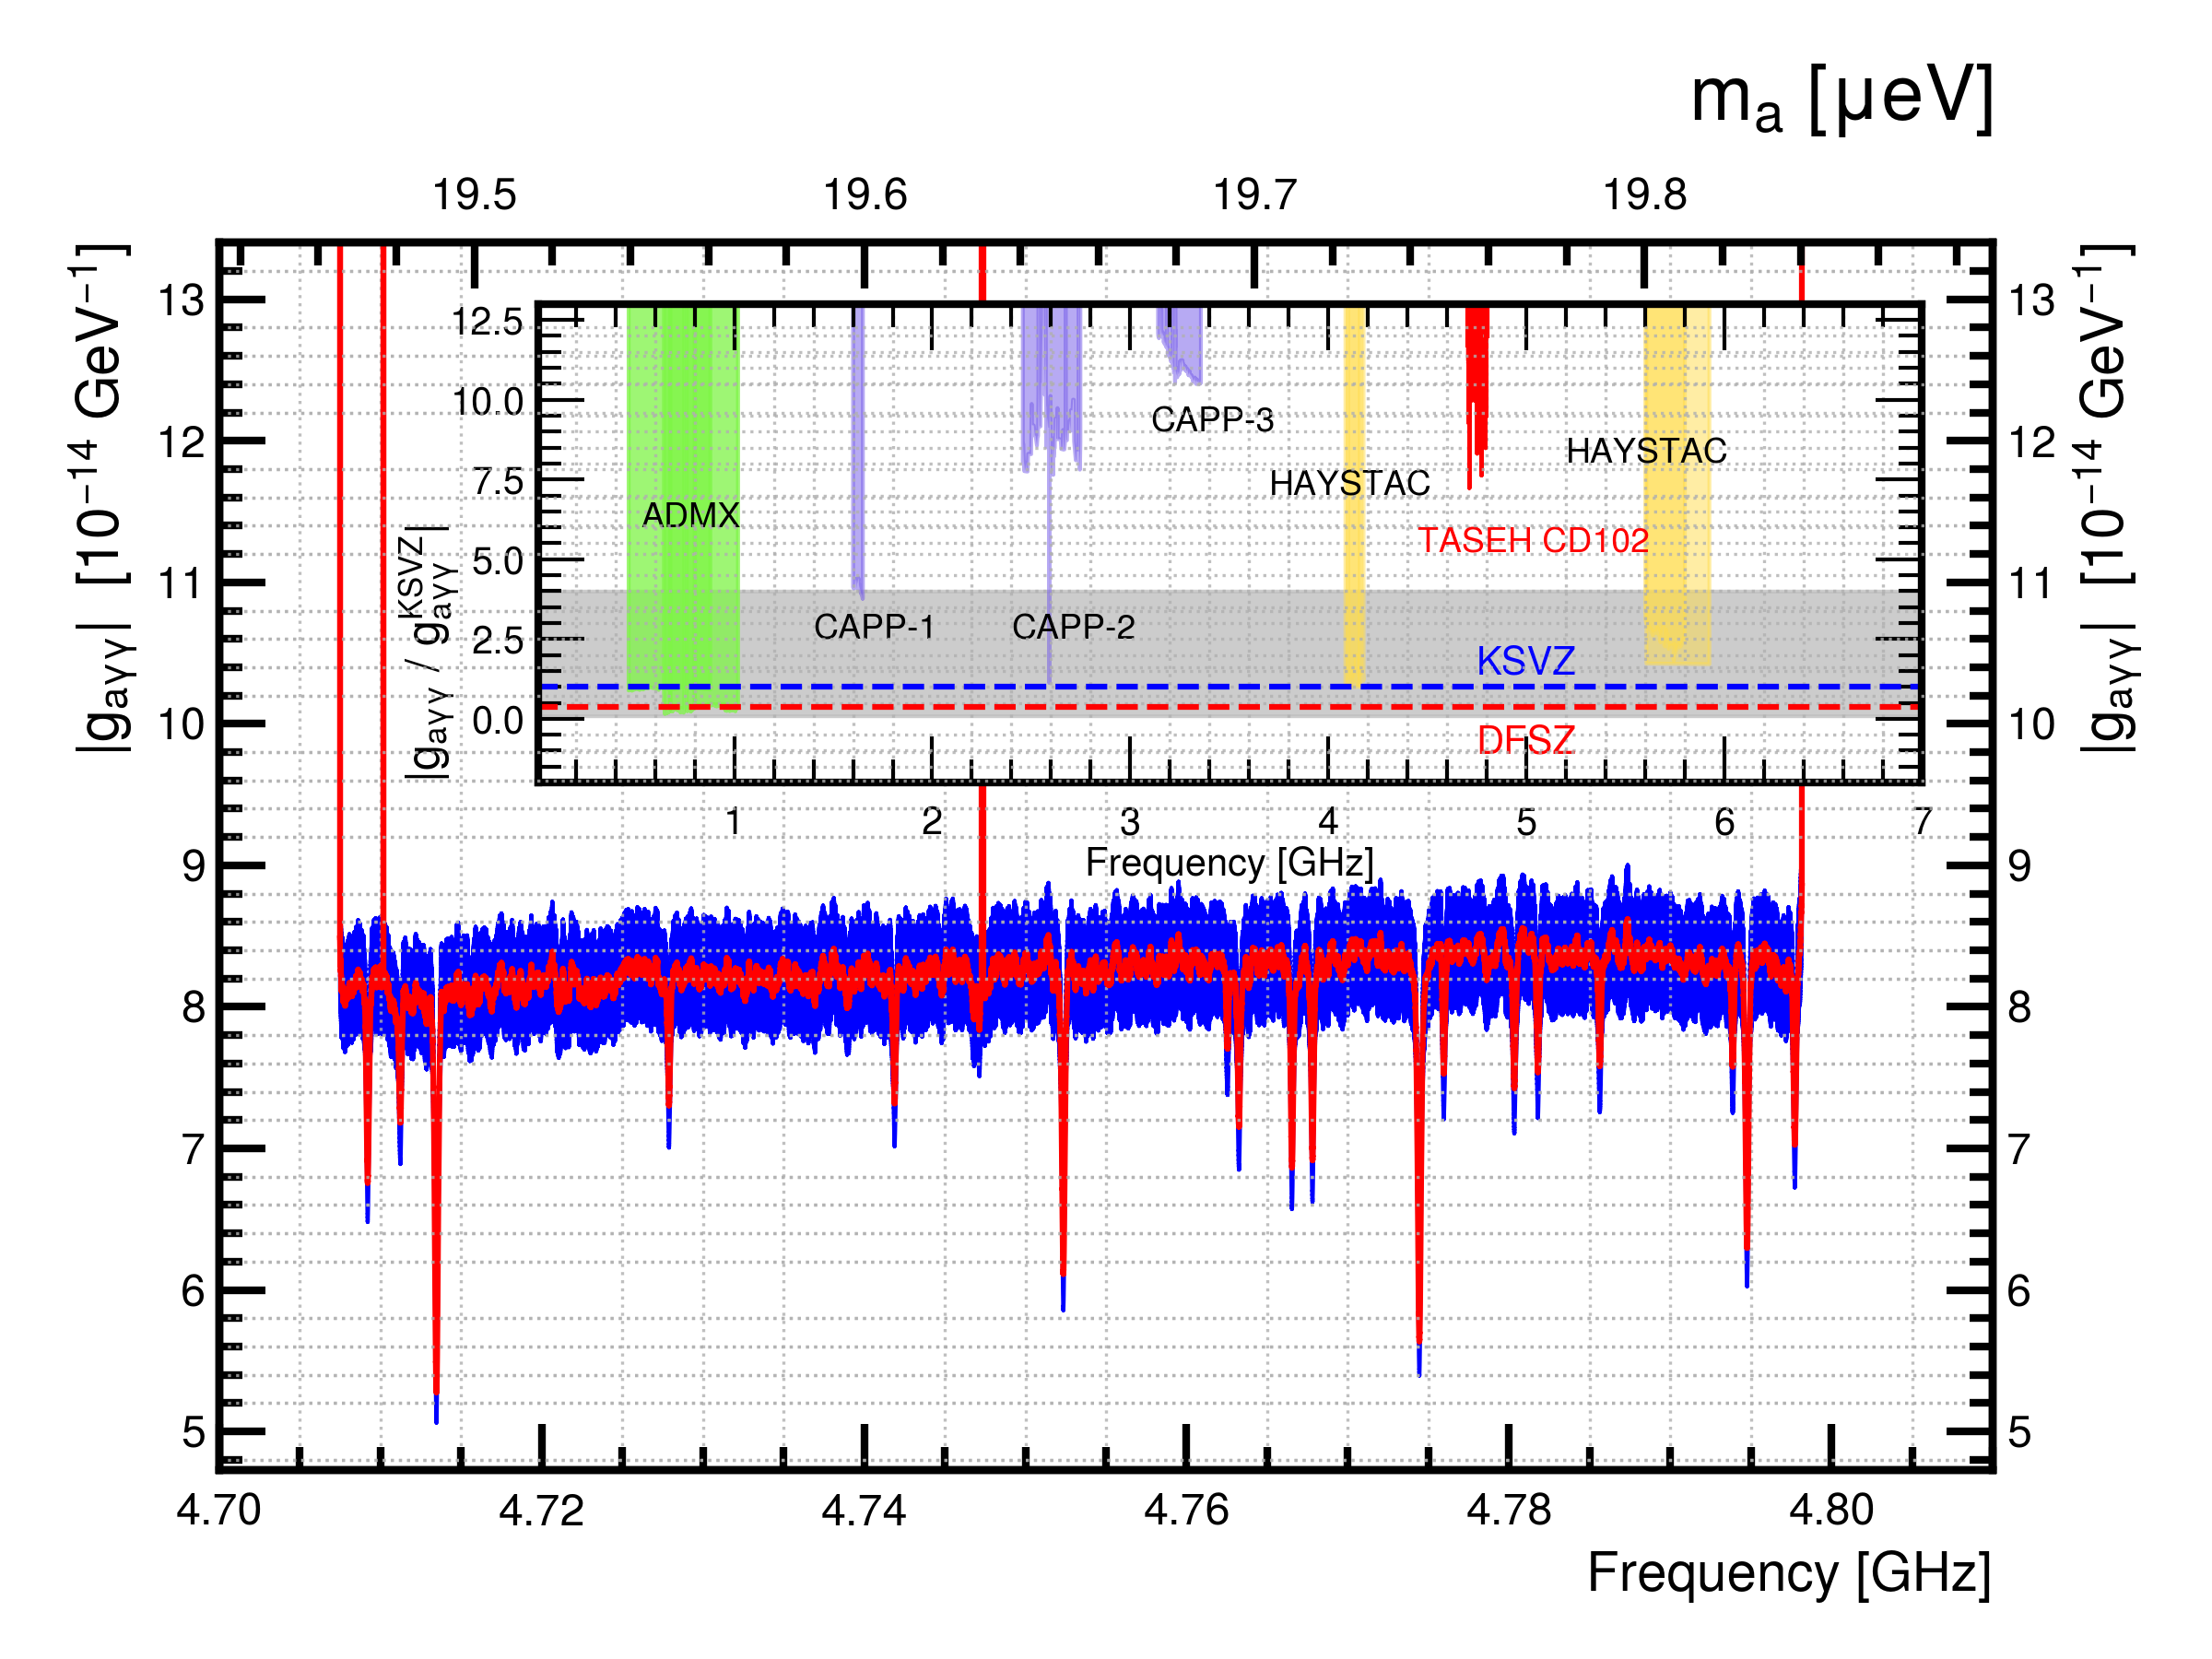
\includegraphics[width=12.9cm]{figures/TASEHonly_limits.png}
  \caption{The limits on \gagg\ and the ratio of the limits on 
\ggamma\ relative to $\left|g_\text{KSVZ}\right|=0.97$ 
  (inset) for the frequency range of 
\flo--\fhi~GHz. The blue error band indicates the systematic 
  uncertainties as discussed in Sec.~\ref{sec:sys}. The yellow 
 band in the inset shows the allowed region of \ggamma\ vs. $m_a$ 
 from various QCD axion models, while the blue and red dashed lines are the 
values predicted by the KSVZ and DFSZ benchmark models, respectively}
  \label{fig:glimit}
\end{figure*}


\begin{figure*} [htbp]
  \centering
 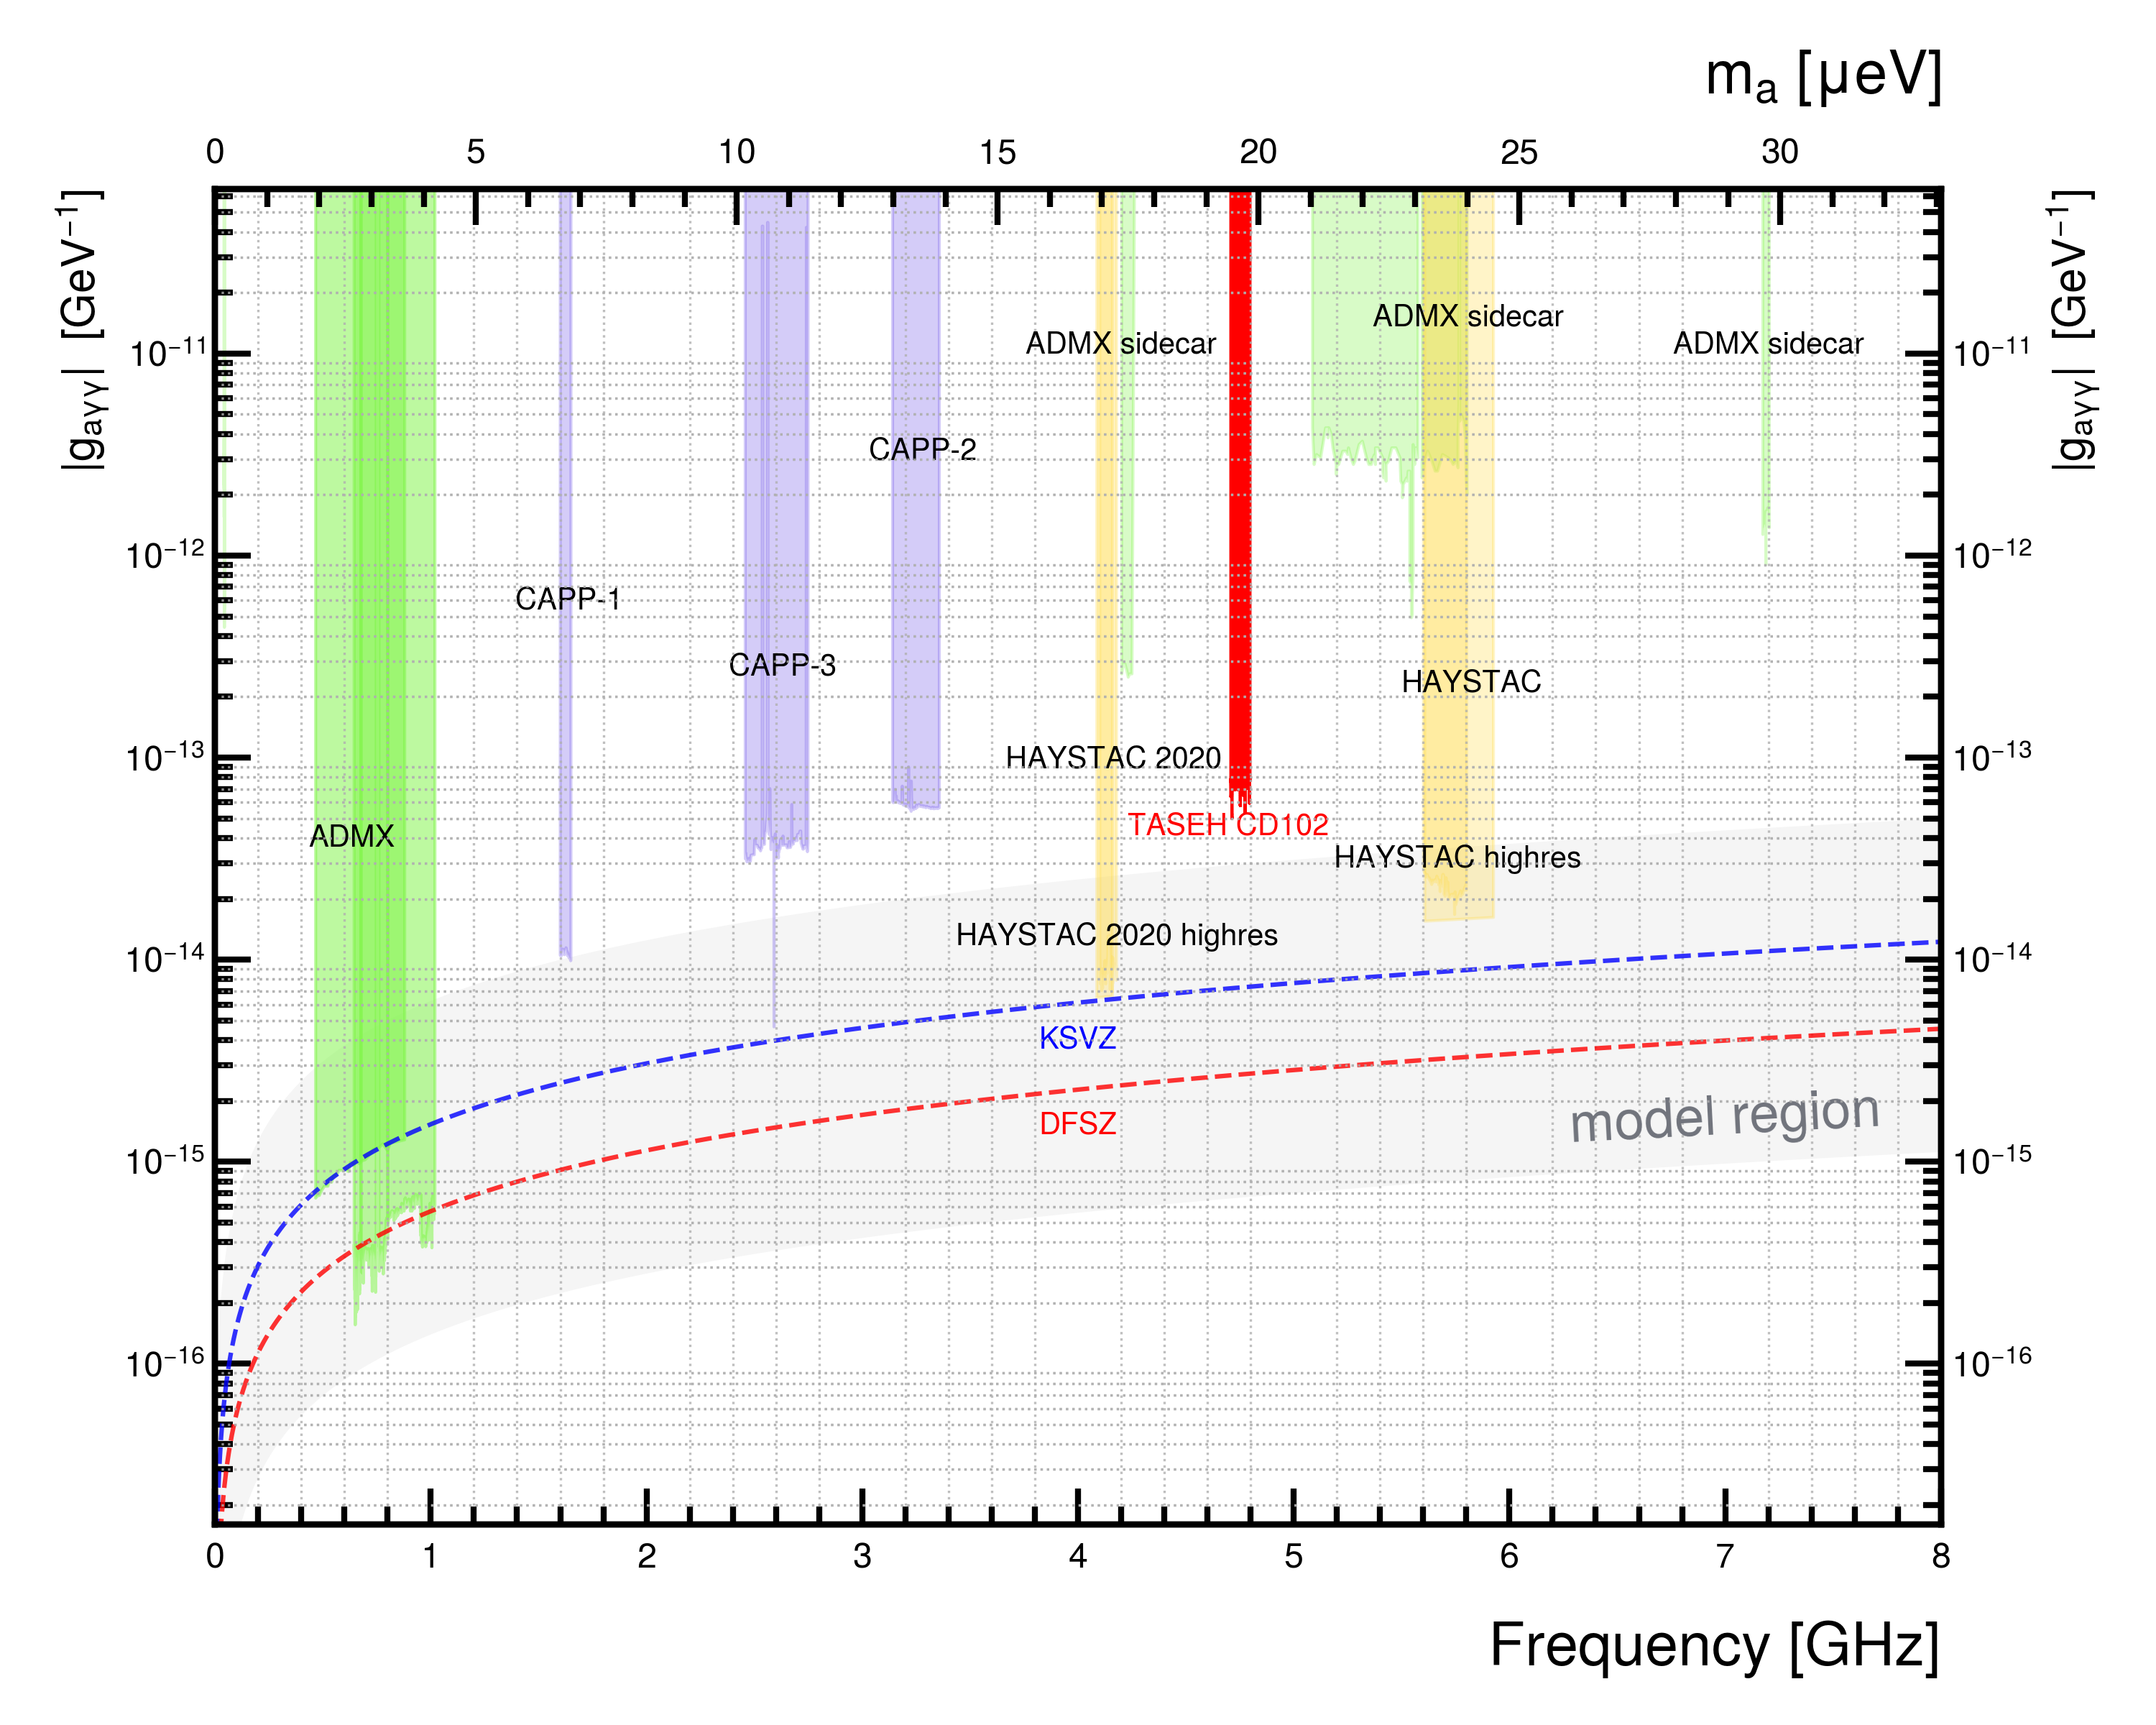
\includegraphics[width=12.9cm]{figures/RealData_limit_allexp.png}
  \caption{The limits on the axion-two-photon coupling \gagg\ for the 
frequency ranges of 0--8~GHz, from the CD102 data of TASEH and previous 
searches performed by the ADMX, CAPP, and HAYSTAC Collaborations. The gray 
band indicates the allowed region of \gagg\ vs. $m_a$ from various QCD axion 
models while the blue and red dashed lines are the values predicted by the 
KSVZ and DFSZ benchmark models, respectively.}
  \label{fig:gaggall}
\end{figure*}




%%%% faxion
After the collection of the CD102 data, 
the synthetic axion signals were injected into the cavity and read out via the 
same transmission line and amplification chain. 
%Due to the uncertainties on the losses of signal transmission
% lines, the synthetic axion signals are not used to perform an absolute 
%calibration of the search sensitivity. Instead, 
%a test with synthetic axion signals could be used to verify the procedures of 
%data acquisition and physics analysis. 
The procedure to generate axion-like signals is summarized in 
Ref.~\cite{TASEHInstrumentation} and the analysis of the synthetic axion 
data is described in Ref.~\cite{TASEHAnalysis}. 
The analysis results of the synthetic axion signals prove that a power 
excess of more than 5$\sigma$ can be found at the expected frequencies via 
the standard analysis procedure.  

%% conclusion 
This Letter presents the first results of a search for axions for the mass 
range $\mlo < \ma < \mhi \muevcc$. 
Apart from the external signals, no candidates with a significance more than
3.355 were found. The experiment excludes models with the 
axion-two-photon coupling $\gagg\gtrsim \avelimit\GeVinv$ at 95\% C.L.,
 a factor of ten 
above the benchmark KSVZ model. The sensitivity on \gagg\ reached by TASEH 
is three orders of magnitude better than the existing limits. 
It is also the first time that a haloscope-type experiment places 
constraints in this mass region. 

%The target of TASEH is to search for axions for the mass range of 
%16.5--20.7\muevcc\ corresponding to a frequency range of 4--5~GHz, with a 
%capability to be extended to 2.5--6~GHz in the future. 
%In the coming years, several upgrades are expected, including: the use of a 
%quantum-limited Josephson parametric amplifier as the first-stage amplifier, 
%the replacement of the existing dilution refrigerator with a new one that has 
%a magnetic field of about 9~Tesla and a larger bore size, and the development 
%of a new cavity with a significantly larger effective volume. 
%With the improvements of the experimental setup and several years of data 
%taking, TASEH is expected to probe the QCD axion band in the target mass range.

\begin{acknowledgments}

\end{acknowledgments}

\bibliography{letter}% Produces the bibliography via BibTeX.

\end{document}
%
% ****** End of file apssamp.tex ******
